\chapter{Usage and Examples}
\section{Procedure}
\begin{itemize}
    \item Clone the repository from \textbf{github} onto your local machine.
    \item Copy your target XML file to the directory of the cloned repository and instantiate an object of \textbf{class ReactionParser} with the filename.
    \item The '\_\_call\_\_' method defined for your convenience allows you to begin the extraction of parameters from the XML file.
    \item In addition to the parameters, information about the Stoichiometric Coefficients and Type of Reaction is derived from the XML File for the reactants and products separately.
    \item The object of \textbf{class Reaction} accepts the parameters extracted from the XML file directly through the \textbf{class ReactionParser}.
    \item The Temperature needs to be provided by the user at run-time through a method 'set\_temperature' of the \textbf{class Reaction}.
    \item The Reaction Rate Coefficient is calculated by calling a method 'compute\_reaction\_rate\_coeff' of \textbf{class Reaction} which instantiates an object of \textbf{class ReactionCoeff} and passes a dictionary of parameters necessary for calculation. 
    \item The \textbf{class ReactionCoeff} consists of methods for individual forms of the Reaction Rate Coefficient and returns the coefficient according to the parameters passed as input.
    \item Finally,  the concentrations of the unique species needs to be provided by the user at run-time through a method 'set\_concentrations' of the \textbf{class Reaction}.
    \item Using the Reaction Rate Coefficent, Unique Specie Concentrations and Stochiometric Coefficients, the Reaction Rate and Progress Rate can be obtained using methods 'compute\_reaction\_rate'  and 'compute\_progress\_rate' defined in the \textbf{class Reaction}.
\end{itemize}
\section{Examples}
\subsection{Case 1 : Single Reaction System}
\textbf{Problem :} \\
Calculate the \textbf{Progress Rate} for a reaction of the following form :
\begin{center}
  $\nu_{A} A + \nu_{B} B \longrightarrow \nu_{C} C.$\\
\end{center}
\\Order your concentration vector so that 
\begin{align}
  \mathbf{x} =
  \begin{bmatrix}
    \left$[ [A] [B] [C] ]^{T}$ \\
  \end{bmatrix}
\end{align}
Test your function with 
\begin{align}
  $\nu_{i}^{\prime}$ =
  \begin{bmatrix}
    \left$[2.0 1.0 0.0]^{T}$ \\
  \end{bmatrix}
\end{align}
And concentrations  
\begin{align}
  $x$ =
  \begin{bmatrix}
    \left$[1.0 2.0 3.0]^{T}$ \\
  \end{bmatrix}
\end{align}
Reaction Rate Coefficent : $k = 10$

\begin{flushleft}
\textbf{Solution Code :}
\end{flushleft}

\begin{mdframed}[backgroundcolor=light-gray, roundcorner=10pt,leftmargin=1, rightmargin=5, innerleftmargin=10, innertopmargin=5,innerbottommargin=5, outerlinewidth=1, linecolor=light-gray]
\begin{lstlisting}
#Copy target XML file into repository
>>> parser(xml_filename)
>>> parser()

#Fetch desired reaction index, in this case 0 (zero)
>>> reac1 = parser.reaction_list[0]

#Print Reaction Equation
>>> print(reac1)

#Set Temperature (although not needed for this)
#reac1.set_temperature(1000)
>>> reac1.set_concentrations({'A':1,'C':3,'B':2})

#Order doesn't matter as long as all species exist
>>> k = reac1.compute_reaction_rate_coef()
>>> omega = reac1.compute_progress_rate()

#Reaction Rate can be calculated similarly
>>> print ("Reaction Rate Coefficient =",k)
>>> print ("Progress Rate =",omega)
\end{lstlisting}
\end{mdframed} 
\textbf{Result :}\\
\\
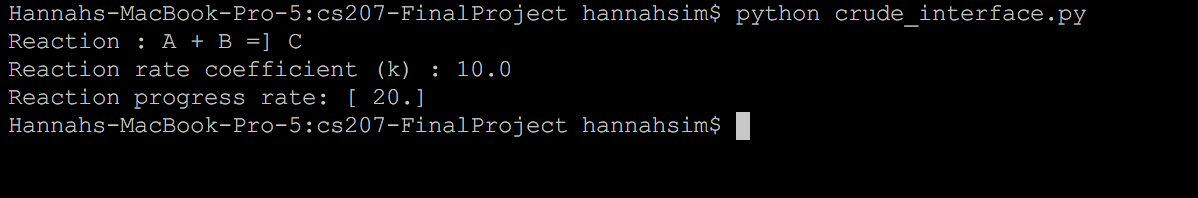
\includegraphics[scale=0.35]{result}